% ============================ 二、问题分析 ============================
\section{问题分析}

\subsection{总体认识}

三问构成一条\textbf{“表征 $\rightarrow$ 归因 $\rightarrow$ 生成”}的递进链条：
问题一把“化学谱 $\rightarrow$ 感官评分”建成高维小样本回归，其产物（可靠的感官
预测器）是问题三评估生成样本感官合理性的\textbf{度量工具}；问题二从同一批数据中
挖出化学--感官的\textbf{因果候选集}，其产物（关键化合物清单）反向约束问题三的
生成方向，使“生成”不至于沦为无意义的随机采样。三问共享同一套数据契约：对数
底数、缺失机制、左删失规则、0--6 分制标定必须在同一处定义一次，否则三问结论
不可相互印证。因此本文先做\\textbf{一次严格的数据审计}（第四章），再依次建模。

技术路线如图~\ref{fig:roadmap} 所示。

\begin{figure}[H]
\centering
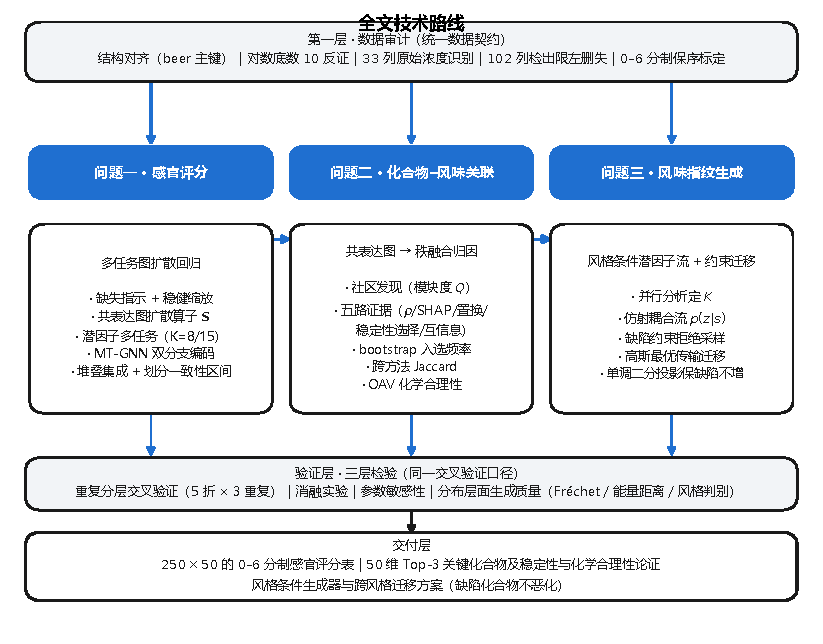
\includegraphics[width=\figw]{images/fig00_roadmap.pdf}
\caption{全文技术路线：审计层统一数据契约，建模层三问共享特征与评估口径，
问题二的归因结果反向约束问题三的生成方向}
\label{fig:roadmap}
\end{figure}

\subsection{问题一的分析}

问题一的数学本质是一个 $\R^{231}\!\rightarrow\!\R^{50}$ 的\textbf{多输出
高维小样本回归}，有三个结构性困难必须分别处理。

\textbf{（1）维数灾难与共线性。}231 个化合物中，萜烯类 65 个、酯类 59 个，同类
化合物之间相关系数常在 0.8 以上（如乙酸乙酯与总酯 $r=0.77$）。这正是普通最小
二乘失效的典型场景：本文实测未加正则的岭回归在留出法下平均
$R^2=-0.45$，比“直接用均值预测”还差。必须用强正则化或特征筛选把有效自由度
压到样本量以下。

\textbf{（2）多任务结构未被利用。}50 个感官维度高度相关（本文实测平均
$|\rho|=0.17$，Aroma 与 Flavour 两套内部同族维度相关可达 0.7 以上）。若为每个
维度独立训练一个模型（这是最直接的做法），等于放弃了“麦芽香-总体”对
“麦芽香-面包”的信息增益。因此本文把它当作\textbf{多任务学习}问题
\cite{caruana1997}，用低秩因子或共享隐层显式共享统计强度。

\textbf{（3）标签噪声与极端值。}感官分是品评小组均值，本身含主观方差；部分啤酒
在“烟熏焦”维度上出现极端高分，会把 $R^2$ 这类平方损失指标严重拉低。这解释了
为什么文献中线性模型在此类数据上会出现\textbf{负 $R^2$}——这不是代码错误，而是
平方损失对长尾标签的固有脆弱性。

据此，问题一的分析策略是：先把特征工程做扎实（缺失插补 + 稳健缩放 + 共表达图
扩散），再在同一交叉验证协议下横向比较“线性 $\rightarrow$ 树模型 $\rightarrow$
潜因子多任务 $\rightarrow$ 图神经网络 $\rightarrow$ 堆叠”五级模型，最后用
分裂一致性给出预测区间，使交付的 0--6 分数\textbf{附带可信度}而非孤立数值。

\subsection{问题二的分析}

问题二要回答的不是“哪些化合物与某感官统计相关”，而是“\textbf{哪些化合物是该
感官的可靠驱动因素}”。二者的差别在于\textbf{稳定性}：231 个特征、250 个样本下，
单次拟合得到的“重要性排序”有很大比例是噪声。因此必须回答三个层次的问题：

\begin{enumerate}[label=(\arabic*),leftmargin=2.2em,itemsep=1pt]
\item \textbf{结构层}：化合物之间存在怎样的共表达模块？同一模块内的化合物往往
  共享代谢通路（如乙酸酯类共用乙酰辅酶 A 前体），这为“Top-3 化学合理性”提供
  了先验——若某感官的 Top-3 恰好落在同一模块，其可信度高于三个孤立化合物。
\item \textbf{归因层}：如何把“重要性”的定义做得不依赖单一模型？本文采用五路
  证据（秩相关、SHAP、置换重要性、稳定性选择、互信息）做秩融合，因为不同方法
  对非线性、交互与共线性的敏感方向不同，融合后结论更稳健。
\item \textbf{验证层}：稳定性用 bootstrap 入选频率与跨方法 Jaccard 双指标量化；
  化学合理性则把 Top-3 还原为“化合物类别 + 代谢来源 + OAV 量级”，并与
  \texttt{6.csv} 给出的独立交叉相关证据对照。
\end{enumerate}

\subsection{问题三的分析}

问题三要求的不只是“生成像样的数”，而是“\textbf{生成符合风格语义、且不引入
缺陷}的化合物谱”，这是一个带约束的条件生成问题。三处风险点决定了建模选择：

\textbf{（1）样本极不平衡。}22 种风格中 Faro 仅 3 款、Brut 4 款。若对每种风格
独立训练生成器，小样本风格必然过拟合。因此必须先降维到潜因子空间，并让各风格
共享协方差结构（收缩估计），使稀有风格向总体“借力”。

\textbf{（2）生成空间必须是化学可行域。}231 维原始化合物空间对 250 个样本而言
过于稀疏，直接在其中做密度估计不可行；而完全不留自由度又退化为“复制训练样本”。
折中方案是在潜因子空间建模密度、再解码回化合物空间，并用\textbf{分布层面的
指标}（而非目视）验证生成质量。

\textbf{（3）跨风格迁移必须显式约束缺陷。}“把 Pils/Lager 变成 Tripel”若只做
朴素插值，会连带把 DMS、双乙酰、4VG 等缺陷一并放大。因此迁移必须写成
\textbf{带约束的优化}：先在潜空间用最优传输给出“风格对齐”的目标点，再沿
源点--目标点连线做单调搜索，取满足缺陷不恶化的最远可行点。这样得到的迁移路径
既可解释（$\lambda$ 越大越像目标风格），又可审计（缺陷单调不增）。
